\documentclass[a4paper, 12pt]{article}

\def\languages{english, french}

%%%%%%%%%%%%%%%%%%% Libraries

%%%%%%%%%% Packages

\usepackage[
backend=biber,
style=numeric-comp,
sorting=none,
maxbibnames=99
]{biblatex}

\newgeometry{margin = 2.5cm}
\makeatletter
\begin{titlepage}
	\begin{minipage}[t][0.425\textheight][t]{\textwidth}
		\begin{center}
		    \ifx\toptitle\undefined
    		    \vfill
    		    \ifx\logopath\undefined
    		    \else
    			    \includegraphics[height=0.2125\textheight]{\logopath}
    			\fi
    		\else
    		    \ifx\logopath\undefined
    		    \else
    			    \includegraphics[height=0.15\textheight]{\logopath}
    			\fi
    			\vfill
    			{\huge \textsc{\toptitle}}
			\fi
			\vfill
		\end{center}
	\end{minipage}
	\vfill
	\begin{minipage}{\textwidth}
		\hspace{0.5em}
		\begin{mdframed}[linewidth = 2pt, innertopmargin = 1em, innerbottommargin = 1em, leftline = false, rightline = false]
			\begin{center}
				{\huge \bfseries \@title}
			\end{center}
		\end{mdframed}
		\hspace{0.5em}
	\end{minipage}
	\vfill
	\begin{minipage}[b][0.425\textheight][t]{\textwidth}
			\ifx\subtitle\undefined
			\else
			    \vspace{-0.5em}
			    \begin{center}
				    {\LARGE \subtitle}
				\end{center}
			\fi
			\vfill
			\ifx\rightauthor\undefined
			    \begin{center}
			        \ifx\authorhead\undefined
			        \else
		                {\large\it \authorhead\\[0.5em]}
		            \fi
			        {\large \@author}
			    \end{center}
			\else
			    \begin{minipage}[t]{0.5\textwidth}
			        \begin{flushleft}
			            \ifx\authorhead\undefined
			            \else
			                {\large\it \authorhead\\[0.5em]}
			            \fi
				        {\large \@author}
				    \end{flushleft}
				\end{minipage}
				\begin{minipage}[t]{0.5\textwidth}
				    \begin{flushright}
				        \ifx\rightauthorhead\undefined
			            \else
			                {\large\it \rightauthorhead\\[0.5em]}
			            \fi
				        {\large \rightauthor}
				    \end{flushright}
				\end{minipage}
			\fi
			\vfill
			\begin{center}
			    \ifx\context\undefined
			    \else
			        {\large \context \\[0.5em]}
			    \fi
			    {\large \@date}
			\end{center}
	\end{minipage}
\end{titlepage}
\makeatother
\restoregeometry
%%%%%%%%%% Packages

\usepackage{float}
\usepackage[skip=1em]{caption}

\usepackage{array}
\usepackage{multirow}
\usepackage{multicol}

%%%%%%%%%% Features

%%%%% Settings

\renewcommand{\arraystretch}{1.2}

%%%%% Commands

\newcommand\noskipcaption[1]{\caption{#1}\vspace{-1em}}
\newcommand\noskipcaptionstar[1]{\caption*{#1}\vspace{-1em}}

%%%%%%%%%% Packages

\usepackage{inconsolata}
\usepackage{listings}

%%%%%%%%%% Features

%%%%% Commands

\newcommand{\Nstyle}[1]{
    \lstdefinestyle{N#1}{
        style=#1,
        %%%%%
        numbers=left
    }
}

\newcommand{\tbFstyle}[1]{
    \lstdefinestyle{tbF#1}{
        style=#1,
        %%%%%
        frame=tb
    }
}

\newcommand{\Fstyle}[1]{
    \lstdefinestyle{F#1}{
        style=#1,
        %%%%%
        frame=single,
        framesep=0em,
        rulesep=0em,
        xleftmargin=0.75em,
        xrightmargin=0.75em,
        framexleftmargin=0.75em,
        framexrightmargin=0.75em,
        framextopmargin=0.5em,
        framexbottommargin=0.5em,
        %%%%%
        numbersep=1.25em
    }
}

\newcommand{\NtbFstyle}[1]{
    \tbFstyle{#1}
    \Nstyle{tbF#1}
}

\newcommand{\NFstyle}[1]{
    \Fstyle{#1}
    \lstdefinestyle{NF#1}{
        style=f#1,
        %%%%%
        xleftmargin=2.75em,
        framexleftmargin=2.75em,
        %%%%%
        numbers=left,
        numbersep=1em
    }
}

%%%%% Styles

\lstdefinestyle{default}{
    breaklines=true,
    breakatwhitespace=true,
    columns=fixed,
	extendedchars=true,
    upquote=true,
	tabsize=4,
    %%%%%
    framerule=0.66pt,
    captionpos=b,
	%%%%%
    basicstyle=\footnotesize\ttfamily,
    numberstyle=\footnotesize\ttfamily,
    showstringspaces=false
}
\Nstyle{default}
\NFstyle{default}
\NtbFstyle{default}

\lstdefinestyle{monokai}{
    style=Fdefault,
    %%%%%
    backgroundcolor=\color[HTML]{272822},
    framerule=0em,
    %%%%%
    basicstyle=\footnotesize\ttfamily\color[HTML]{f8f8f2},
    numberstyle=\footnotesize\ttfamily\color[HTML]{272822},
    commentstyle=\color[HTML]{75715e},
    keywordstyle=[1]{\color[HTML]{f92672}},
    keywordstyle=[2]{\color[HTML]{A6E22E}},
    keywordstyle=[3]{\color[HTML]{ae81ff}},
    stringstyle=\color[HTML]{e6db74},
    %%%%%
    % otherkeywords={!,.,+,-,*,/,=,<,>,^,|,\&,OR,AND}
}

\lstdefinestyle{Nmonokai}{
    style=monokai,
    %%%%%
    xleftmargin=2.75em,
    framexleftmargin=2.75em,
    %%%%%
    numbers=left,
    numberstyle=\footnotesize\ttfamily\color[HTML]{f8f8f2},
    numbersep=1em
}

\lstdefinestyle{c}{
    language=C,
    style=default,
    %%%%%
    commentstyle=\color[HTML]{228B22},
    keywordstyle=\color[HTML]{0000FF},
    stringstyle=\color[HTML]{A020F0},
    emphstyle=\color[HTML]{0000FF},
    %%%%%
    emph={}
}

\lstdefinestyle{cpp}{
    language=C++,
    style=default,
    %%%%%
    commentstyle=\color[HTML]{228B22},
    keywordstyle=\color[HTML]{0000FF},
    stringstyle=\color[HTML]{A020F0},
    emphstyle=\color[HTML]{0000FF},
    %%%%%
    emph={std}
}

\lstdefinestyle{matlab}{
    language=matlab,
    style=default,
    %%%%%
    basicstyle=\footnotesize\fontfamily{pcr}\selectfont,
    numberstyle=\footnotesize\fontfamily{pcr}\selectfont,
    commentstyle=\color[HTML]{228B22},
    keywordstyle=\color[HTML]{0000FF},
    stringstyle=\color[HTML]{A020F0},
    emphstyle=\color[HTML]{0000FF},
    %%%%%
    emph={clearvars}
}

\lstdefinestyle{python}{
    language=python,
    style=default,
    %%%%%
    commentstyle=\color[RGB]{221,0,0},
    keywordstyle=[1]{\color[RGB]{255,119,0}},
    keywordstyle=[2]{\color[RGB]{144,0,144}},
    stringstyle=\color[RGB]{0,170,0},
    emphstyle=\color[RGB]{255,119,0},
    %%%%%
    emph={}
}

\lstdefinestyle{java}{
    language=java,
    style=default,
    %%%%%
    commentstyle=\color[HTML]{228B22},
    keywordstyle=\color[HTML]{0000FF},
    stringstyle=\color[HTML]{A020F0},
    emphstyle=\color[HTML]{0000FF},
    %%%%%
    emph={}
}

%%%%%%%%%% Packages

\usepackage{amsmath}
\usepackage{amssymb}
\usepackage{bm}
\usepackage{esint}
\usepackage[makeroom]{cancel}

%%%%%%%%%% Features

%%%%% Macros

\newcommand{\rbk}[1]{\left(#1\right)}
\newcommand{\cbk}[1]{\left\{#1\right\}}
\newcommand{\sbk}[1]{\left[#1\right]}
\newcommand{\abs}[1]{\left|#1\right|}
\newcommand{\norm}[1]{\left\|#1\right\|}

\newcommand{\fact}[1]{#1!}
\newcommand{\e}[1]{\mathbf{e}_{#1}}
\newcommand{\deriv}{\mathrm{d}}
\DeclareMathOperator{\tr}{tr}

\def\Rl{\mathbb{R}}
\def\Cx{\mathbb{C}}
\def\Na{\mathbb{N}}
\def\Zi{\mathbb{Z}}

%%%%%%%%%% Packages

\usepackage{amsthm}
\usepackage{thmtools}

%%%%%%%%%% Features

%%%%% Settings

\makeatletter
\define@key{thmdef}{mdthm}[{}]{
	\thmt@trytwice{\def\thmt@theoremdefiner{\mdtheorem[#1]}}{}}
\makeatother

\begingroup
\makeatletter
\@for\theoremstyle:=plain,definition,remark\do{
	\expandafter\g@addto@macro\csname th@\theoremstyle\endcsname{
		\addtolength\thm@preskip\parskip
	}
}
\endgroup

\renewcommand{\qedsymbol}{$\blacksquare$}

% language

\ifx\lgthm\undefined
	\def\lgthm{Theorem}
	\def\lgprf{Proof}
	\def\lglem{Lemma}
	\def\lgprop{Proposition}
	\def\lgdefn{Definition}
	\def\lghyp{Hypothesis}
	\def\lgmeth{Method}
	\def\lgquest{Question}
	\def\lgansw{Answer}
	\def\lgexpl{Example}
	\def\lgrmk{Remark}
	\def\lgnote{Note}
	\def\lgtip{Tip}
\fi

%%%%% Commands

\newcommand\qedadd{\pushQED{\qed}\popQED}

%%%%% Environments

\theoremstyle{plain}
\newtheorem{thm}{\lgthm}
\newtheorem{lem}[thm]{\lglem}
\newtheorem{prop}[thm]{\lgprop}

\theoremstyle{definition}
\newtheorem{defn}{\lgdefn}
\newtheorem{hyp}{\lghyp}
\newtheorem{meth}{\lgmeth}
\newtheorem{quest}{\lgquest}

\theoremstyle{remark}
\newtheorem{answ}{\lgansw}[quest]
\newtheorem{expl}{\lgexpl}
\newtheorem*{rmk}{\lgrmk}
\newtheorem*{note}{\lgnote}
\newtheorem*{tip}{\lgtip}

% framed

\mdfdefinestyle{thicc}{
	nobreak=true,
	skipabove=\topskip,
	skipbelow=\topskip,
	innerleftmargin=0.5em,
	innerrightmargin=0.5em,
	innerbottommargin=0.5em,
	innertopmargin=0.5em,
	linewidth=0.25em,
	roundcorner=0.15em,
	linecolor=black!10,
	frametitlebackgroundcolor=black!10,
	theoremseparator={.}
}

\declaretheorem[mdthm={style=thicc, linecolor=red!20, frametitlebackgroundcolor=red!20}, sibling=thm, name=\lgthm]{framedthm}
\declaretheorem[mdthm={style=thicc, linecolor=red!20, frametitlebackgroundcolor=red!20}, sibling=thm, name=\lglem]{framedlem}
\declaretheorem[mdthm={style=thicc, linecolor=blue!20, frametitlebackgroundcolor=blue!20}, sibling=thm, name=\lgprop]{framedprop}
\declaretheorem[mdthm={style=thicc, nobreak=false}, parent=thm, name=\lgprf]{framedprf}

\declaretheorem[mdthm={style=thicc, linecolor=black!20!green!20, frametitlebackgroundcolor=black!20!green!20}, sibling=defn, name=\lgdefn]{frameddefn}
\declaretheorem[mdthm={style=thicc, linecolor=blue!20, frametitlebackgroundcolor=blue!20}, sibling=hyp, name=\lghyp]{framedhyp}
\declaretheorem[mdthm={style=thicc}, name=\lgmeth]{framedmeth}
\declaretheorem[mdthm={style=thicc, linecolor=orange!20, frametitlebackgroundcolor=orange!20}, sibling=quest, name=\lgquest]{framedquest}

\declaretheorem[mdthm={style=thicc, nobreak=false}, sibling=answ, name=\lgansw]{framedansw}
\declaretheorem[mdthm={style=thicc, nobreak=false}, sibling=expl, name=\lgexpl]{framedexpl}

%%%%%%%%%% Packages

\usepackage{siunitx}

%%%%%%%%%% Features

%%%%% Settings

\ifx\decimalsign\undefined
\else
    \sisetup{output-decimal-marker = \decimalsign}
\fi


%%%%% Settings

% lists
\frenchbsetup{StandardLists=true}

% units
\def\decimalsign{,}

% captions
\addto\captionsfrench{\def\figurename{Figure}}
\addto\captionsfrench{\def\tablename{Table}}
\addto\captionsfrench{\def\proofname{Preuve}}

% theorems

\def\lgthm{Théorème}
\def\lgprf{Preuve}
\def\lglem{Lemme}
\def\lgprop{Proposition}
\def\lgdefn{Définition}
\def\lghyp{Hypothèse}
\def\lgmeth{Méthode}
\def\lgquest{Question}
\def\lgansw{Réponse}
\def\lgexpl{Exemple}
\def\lgrmk{Remarque}
\def\lgnote{Note}
\def\lgtip{Conseil}

%%%%% Macros

\def\tq{\text{t.q.}}
\def\cad{c.-à-d.}
\def\Cad{C.-à-d.}


\usepackage{listingsutf8}

%%%%%%%%%%%%%%%%%%% Titlepage

\def\logopath{resources/pdf/logo-uliege.pdf}
\def\toptitle{Université de Liège}
\title{Projet (partie 2)}
\def\subtitle{Bases de données}
%\def\authorhead{Author}
\author{
    Sabrina \textsc{Bonghi} (20161420)\\
    Maxime \textsc{Meurisse} (20161278)\\
    Valentin \textsc{Vermeylen} (20162864)\\
}
%\def\rightauthorhead{}
%\def\rightauthor{}
\def\context{3\ieme{} année de Bachelier Ingénieur civil}
\date{Année académique 2018-2019}

%%%%%%%%%%%%%%%%%%%

\fancyhead[R]{}

\hypersetup {
    colorlinks=true,
    urlcolor=blue
}

\NFstyle{default}

\lstdefinestyle{sql}{
    language=SQL,
    style=NFdefault,
    %%%%%
    commentstyle=\color[HTML]{228B22},
    keywordstyle=\color[HTML]{0000FF},
    stringstyle=\color[HTML]{A020F0},
    emphstyle=\color[HTML]{0000FF},
    %%%%%
    emph={}
}

\lstdefinestyle{php}{
    language=PHP,
    style=NFdefault,
    %%%%%
    commentstyle=\color[HTML]{228B22},
    keywordstyle=\color[HTML]{0000FF},
    stringstyle=\color[HTML]{A020F0},
    emphstyle=\color[HTML]{0000FF},
    %%%%%
    emph={}
}

\lstset{inputencoding=utf8/latin1}

%%%%%%%%%%%%%%%%%%%

\begin{document}
	\newgeometry{margin = 2.5cm}
\makeatletter
\begin{titlepage}
	\begin{minipage}[t][0.425\textheight][t]{\textwidth}
		\begin{center}
		    \ifx\toptitle\undefined
    		    \vfill
    		    \ifx\logopath\undefined
    		    \else
    			    \includegraphics[height=0.2125\textheight]{\logopath}
    			\fi
    		\else
    		    \ifx\logopath\undefined
    		    \else
    			    \includegraphics[height=0.15\textheight]{\logopath}
    			\fi
    			\vfill
    			{\huge \textsc{\toptitle}}
			\fi
			\vfill
		\end{center}
	\end{minipage}
	\vfill
	\begin{minipage}{\textwidth}
		\hspace{0.5em}
		\begin{mdframed}[linewidth = 2pt, innertopmargin = 1em, innerbottommargin = 1em, leftline = false, rightline = false]
			\begin{center}
				{\huge \bfseries \@title}
			\end{center}
		\end{mdframed}
		\hspace{0.5em}
	\end{minipage}
	\vfill
	\begin{minipage}[b][0.425\textheight][t]{\textwidth}
			\ifx\subtitle\undefined
			\else
			    \vspace{-0.5em}
			    \begin{center}
				    {\LARGE \subtitle}
				\end{center}
			\fi
			\vfill
			\ifx\rightauthor\undefined
			    \begin{center}
			        \ifx\authorhead\undefined
			        \else
		                {\large\it \authorhead\\[0.5em]}
		            \fi
			        {\large \@author}
			    \end{center}
			\else
			    \begin{minipage}[t]{0.5\textwidth}
			        \begin{flushleft}
			            \ifx\authorhead\undefined
			            \else
			                {\large\it \authorhead\\[0.5em]}
			            \fi
				        {\large \@author}
				    \end{flushleft}
				\end{minipage}
				\begin{minipage}[t]{0.5\textwidth}
				    \begin{flushright}
				        \ifx\rightauthorhead\undefined
			            \else
			                {\large\it \rightauthorhead\\[0.5em]}
			            \fi
				        {\large \rightauthor}
				    \end{flushright}
				\end{minipage}
			\fi
			\vfill
			\begin{center}
			    \ifx\context\undefined
			    \else
			        {\large \context \\[0.5em]}
			    \fi
			    {\large \@date}
			\end{center}
	\end{minipage}
\end{titlepage}
\makeatother
\restoregeometry
	\section{Architecture du site web}
	\label{sec:architecture}
	La version définitive du site web est disponible via l'URL :
	\begin{center}
	    \href{http://www.student.montefiore.ulg.ac.be/~s161278/}{\texttt{student.montefiore.ulg.ac.be/\textasciitilde s161278/}}
	\end{center}
	Les identifiants de connexion sont identiques à ceux de la base de données, à savoir :
	\begin{itemize}
	    \item Nom d'utilisateur : {\bf group1}
	    \item Mot de passe : {\bf co/A/vp7qq}
	\end{itemize}
	L'arborescence des fichiers composant le site web est présentée à la figure \ref{fig:arborescence}.
	\begin{figure}[H]
	    \centering
	    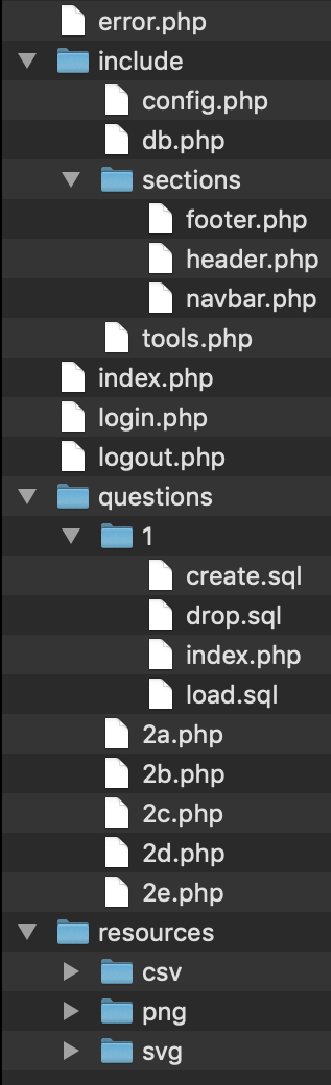
\includegraphics[scale=0.6]{resources/pdf/arborescence.pdf}
	    \caption{Arborescence des fichiers composant le site web}
	    \label{fig:arborescence}
	\end{figure}
	Le site web se compose donc de plusieurs fichiers et dossiers.\par
	Le dossier \texttt{resources} contient les ressources du site web, à savoir les icônes et logos utilisés (en format \texttt{png} et \texttt{svg}, situés dans les dossiers du même nom) ainsi que tous les fichiers \texttt{csv} contenant les données de la base de données.\par
	Le dossier \texttt{questions} contient les fichiers \texttt{PHP} contenant les requêtes \texttt{SQL} (ainsi que le traitement des données en \texttt{PHP} et la structure de la page web en \texttt{HTML}) répondant aux différentes questions posées. Le fichier porte le nom de la question à laquelle il répond. Pour la question 1, il s'agit d'un dossier contenant trois fichiers \texttt{SQL} et un fichier \texttt{PHP} répondant à la question.\par
	Le dossier \texttt{include} contient des fichiers contenant des bouts de code (variables, méthodes et mise en forme \texttt{HTML}) qui sont utilisés à plusieurs endroits du site web. En particulier, les fichiers se trouvant dans le dossier \texttt{sections} contiennent du code \texttt{HTML} de mise en forme qui sert de base à toutes les pages visitables du site web. Le fichier \texttt{tools.php} contient des méthodes \texttt{PHP} utiles, notamment celle vérifiant si un utilisateur est connecté ou non au site web. Le fichier \texttt{db.php} contient le script \texttt{PHP} permettant de se connecter à la base de données.\par
	Les fichiers \texttt{login.php} et \texttt{logout.php} permettent la connexion et déconnexion du site web via des scripts \texttt{PHP} et formulaire \texttt{HTML}.\par
	Le fichier \texttt{error.php} permet d'afficher les erreurs (notamment les erreurs 400, 401, 403, 404 et 500) de manière personnalisée.\par
	Finalement, le fichier \texttt{.htaccess} permet de modifier certaines propriétés du site web, en particulier la ré-écriture d'URL (afin d'accéder à un fichier sans devoir renseigner son extension) et les redirections vers la page d'erreur personnalisée.
	\section{Initialiser la base de données}
	Les requêtes \texttt{SQL} permettant d'initialiser la base de données se trouvent dans les fichiers \texttt{create.sql} et \texttt{load.sql} (dans le dossier \texttt{1/}, lui-même dans le dossier \texttt{questions/}). Ces requêtes sont appelées dans le fichier \texttt{index.php} du même dossier.\par
	Pour initialiser la base de données, il suffit de suivre les étapes suivantes :
	\begin{framedmeth*}[Initialisation de la base de données]
    	\begin{enumerate}
    	    \item Se rendre sur l'URL :
    	    \begin{center}
    	        \href{http://www.student.montefiore.ulg.ac.be/\textasciitilde s161278/questions/1/}{\texttt{student.montefiore.ulg.ac.be/~s161278/questions/1/}}
    	    \end{center}
    	    \item Cliquer sur le bouton vert \og Initialiser la base de données\fg{}.
    	\end{enumerate}
    \end{framedmeth*}
    Contrairement aux autres requêtes \texttt{SQL}, celles-ci peuvent être exécutées sans devoir être connecté au site web.\par
    Il existe aussi une requête \texttt{SQL} permettant de supprimer toutes les tables (fichier \texttt{drop.sql}). Elle peut être exécutée via la même page que la requête d'initialisation et permet, en combinaison avec l'autre requête, de réinitialiser la base de données, \cad{} recréer les tables avec les valeurs d'origine fournies dans les fichiers \texttt{csv}.
	\section{Les requêtes SQL}
	Comme présenté à la section \ref{sec:architecture}, toutes les requêtes \texttt{SQL} (exceptées celles de l'initialisation de la base de données) répondant aux différentes questions se trouvent dans les fichiers \texttt{PHP} du dossier \texttt{questions}.\par
	Ces différentes requêtes, isolées du reste et remises au clair, sont reprises ci-après.
	\subsection{Question 1}
	On remarque que le code \texttt{SQL} permettant de charger le contenu de la table articles convertit l'attribut \texttt{date\_publication} en format \texttt{DATE}. Pour ce faire, on utilise la méthode \texttt{STR\_TO\_DATE} de \texttt{SQL} (car la date dans le fichier \texttt{csv} n'était pas dans un format de date standard).\par
	L'avantage de cette conversion est qu'il sera beaucoup plus simple de trier les dates (par ordre croissant ou décroissant) par la suite (en effet, un simple \texttt{ORDER BY date\_publication ASC/DESC} suffira).
	\lstinputlisting[style=sql, caption={Requ\^ete \texttt{SQL} de la question 1}]{resources/sql/1.sql}
	\subsection{Question 2a}
	Cette requête a été construite en \texttt{PHP}. En effet, selon les contraintes de recherche renseignées ou non par l'utilisateur, la requête n'est pas la même.\par
	Dans ce script, la variable \texttt{tab\_constraints} est un tableau contenant toutes les contraintes renseignées par l'utilisateur. Chaque contrainte est sous forme d'un tableau où le premier élément est l'attribut et le second sa valeur.\par
	L'utilisation de \texttt{COLLATE UTF8\_GENERAL\_CI} juste avant le mot clé \texttt{LIKE} dans les contraintes de contenance permet de ne pas tenir compte de la casse lors de la recherche.
	\lstinputlisting[style=php, caption={Requ\^ete \texttt{SQL}, construite en \texttt{PHP}, de la question 2a}]{resources/php/2a.php}
	\subsection{Question 2b}
	Dans cette requête, le \texttt{x} correspond au matricule du premier auteur, renseignée par l'utilisateur.
	\lstinputlisting[style=sql, caption={Requ\^ete \texttt{SQL} de la question 2b}]{resources/sql/2b.sql}
	\subsection{Question 2c}
	Cette requête, assez longue, a été construite en \texttt{PHP}. En effet, les requêtes d'ajout dépendent des données renseignées ou non et du type de l'article.\par
	Les requêtes permettant de vérifier les entrées de l'utilisateur n'ont pas été reprises ci-après.\par
	Chaque variable portant le nom d'un attribut contient la valeur de cet attribut (renseignée par l'utilisateur).\par
	L'utilisation des méthodes de \texttt{PDO} concernant les transactions permettent d'assurer la cohérence de la base de données, même en cas d'erreur lors de l'insertion. En effet, il serait inacceptable qu'une partie des données soit insérée dans une table mais que le reste des données ne soit pas insérée à cause d'une erreur. Avec la gestion des transactions, cette situation ne peut pas arriver : soit toutes les données sont insérées, soit rien n'est inséré.\par
	Pour ce faire, lorsque toutes les données de l'utilisateur ont été traitées, on démarre une transaction (grâce à la méthode correspondante de \texttt{PDO}) et on verrouille en écriture toutes les tables dans lesquelles on va rajouter des données. On tente d'ajouter les données. Si aucune erreur n'est survenue, on effectue un {\it commit}, sinon on effectue un {\it rollback} (grâce aux méthodes correspondantes de \texttt{PDO}). Dans tous les cas, on déverouille les tables.
	\lstinputlisting[style=php, caption={Requ\^ete \texttt{SQL}, construite en \texttt{PHP}, de la question 2c}]{resources/php/2c.php}
	\subsection{Question 2d}
	Cette requête \texttt{SQL} se compose de plusieurs types de \texttt{JOIN} imbriqués.\par
	Le premier \texttt{NATURAL JOIN} entre \texttt{T1} et \texttt{T2} (et renommé \texttt{T3}) permet de récupérer les participations aux conférences de chaque auteur.\par
	Le deuxième \texttt{NATURAL JOIN} entre \texttt{T1} et \texttt{T2} (et renommé \texttt{T4}) permet de récupérer les auteurs de chaque article de conférence.\par
	Le \texttt{LEFT JOIN} entre \texttt{T3} et \texttt{T4} permet d'associer à chaque auteur ayant participé à une conférénce l'(les) article(s) qu'il y a écrit. Le \texttt{LEFT JOIN} permet de conserver la participation d'un auteur à une conférence même s'il n'y a pas écrit d'article.\par
	Il suffit ensuite de sélectionner les auteurs qui, pour chacune de leur participation à une conférence, ont au moins un article associé.
	\lstinputlisting[style=sql, caption={Requ\^ete \texttt{SQL} de la question 2d}]{resources/sql/2d.sql}
	\subsection{Question 2e}
	Cette requête \texttt{SQL} se compose de plusieurs \texttt{NATURAL JOIN} imbriqués.\par
	Le premier (entre \texttt{T1} et \texttt{T2}) a pour but de récupérer les URL des articles ayant été écrits aux 5 conférences les plus populaires depuis 2012.\par
	Le deuxième (entre \texttt{T3} et \texttt{T4}) a pour but de récupérer les sujets de tous ces articles.\par
	Il suffit ensuite de sélectionner ces sujets, compter le nombre de fois que chaque sujet apparait et les classer par ordre décroissant d'apparition.
	\paragraph{Remarque} Les résultats de cette requête, affichée sur la page \texttt{PHP} correspondante, ne sont pas toujours identiques. Cela vient du fait que les 5\ieme{} et 6\ieme{} conférences les plus populaires ont la même cote de popularité. Dès lors, on suppose que \texttt{SQL} effectue un choix arbitraire entre ces deux conférences pour sélectionner les 5 conférences les plus populaires. Ce choix arbitraire peut donc mener à des résultats différents pour plusieurs exécutions du même script.
	\lstinputlisting[style=sql, caption={Requ\^ete \texttt{SQL} de la question 2e}]{resources/sql/2e.sql}
\end{document}
